\chapter{椭圆型方程的差分方法}

\section{一个典型例子}

\begin{instance}
    如图所示，给定一个各向同性均匀的金属杆，其侧面绝热，有热源作用，求热平衡时的温度分布. \par
    \begin{figure}[H]
        \centering
        \vspace{-1.5 em}
        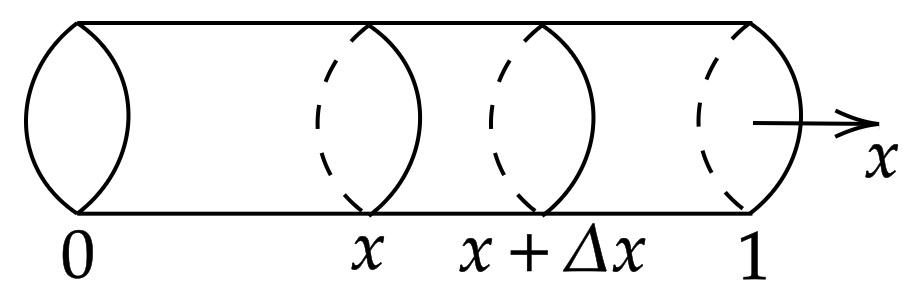
\includegraphics[width=0.4\textwidth]{fig/1.1.png}
        \captionof{figure}{热传导示意图}
        \vspace{-1 em}
    \end{figure}
    我们的目标是对其数学建模.
    \begin{enumerate}[label=Step \arabic*., leftmargin=4em]
        \item \textbf{符号引进}\par
        $u(x)$：$x$时刻的温度 \\
        $S$：截面面积 \\ 
        $k$：热传导系数 \\
        $f(x)$：热源密度
        \item \textbf{建立微分方程方程模型}
        \begin{enumerate}[label=(\arabic*), leftmargin=2em]
            \item 热物理的基本假设 \par
            Fourier热传导定律：$\d Q=-k\partial_nu\d S\d t$
            \begin{figure}[H]
                \centering
                \vspace{-1.5 em}
                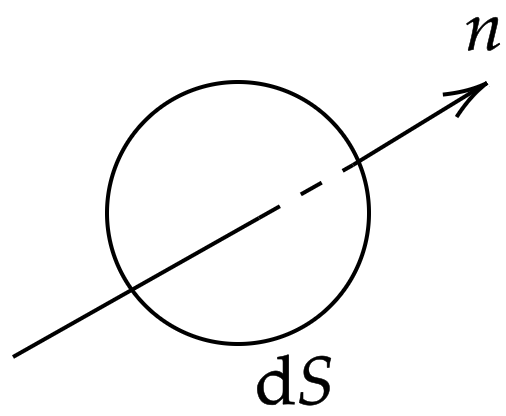
\includegraphics[width=0.2\textwidth]{fig/1.2.png}
                \captionof{figure}{}
                \vspace{-1 em}
            \end{figure}
            \item 使用微元法建模 \par
            在单位时间，考虑微元$[x,x+\Delta x]$的热量变化.\par
            产生的热量为$\Delta Q=f(x)\Delta x S$，流出的热量为$\Delta Q'=-ku'(x+\Delta x)S+ku'(x)S$\par
            由能量守恒定律，$\Delta Q=\Delta Q'$，即$f(x)\Delta x S=-(ku')(x+\Delta x)S+(ku')(x)S$\par
            $\Rightarrow \frac{(ku')(x+\Delta x)-(ku')(x)}{\Delta x}=f(x)$\par
            令$\Delta x\to 0$，$-(ku')'(x)=f(x),0<x<1$\par
            除此之外，对于边界无法使用微元法，因此需要引入边界条件.
            \begin{subequations}
            \begin{empheq}[left=\empheqlbrace]{align}
                &-(ku')'(x)=f(x),0<x<1\\
                &u(0)=u(1)=0
            \end{empheq}
            \end{subequations}
        \end{enumerate}
    \end{enumerate}\par
    问题是能否得到(1.1a)-(1.1b)的显式解？\par
    为了方便计算，设$k(x)=k=1$，则上述方程可以简化为
    \begin{subequations}
            \begin{empheq}[left=\empheqlbrace]{align}
                &-u''(x)=f(x),0<x<1\\
                &u(0)=u(1)=0
            \end{empheq}
    \end{subequations}\par
    对第一个式子作积分，可得$u'(x)=u'(0)-\int_0^xf(s)\d s$.\par
    再作积分可得$u(x)=u(0)+\int_0^x\left(u'(0)-\int_0^sf(t)\d t\right)\d s$.\par
    由$u(0)=0$，$u(x)=u'(0)x-\int_0^x\int_0^s f(t)\d t\d s=u'(0)x-\int_0^x(x-s)f(s)\d s$.\par
    由$u(1)=0$知$u'(0)=\int_0^1(1-s)f(s)\d s$.\par
    令$\chi_{[0,x]}(s)=\begin{cases}
    1,0\leq s\leq x \\
    0,x<s\leq 1
    \end{cases}$，那么$u(x)=\int_0^1\left((1-s)x-\chi_{[0,x]}(s)(x-s)\right)f(s)\d s$.\par
    再记$K(x,s)=(1-s)x-\chi_{[0,x]}(s)(x-s)=\begin{cases}
    (1-x)s,0\leq s\leq x \\
    (1-s)x, x<s\leq 1
    \end{cases}$，则$u(x)=\int_0^1K(x,s)f(s)\d s$.\par
    由此我们得到了问题的显式解.\par
\end{instance}
\begin{note}
        上面给出的$K(x,s)$被称为Green函数，它满足$\begin{cases}
            -K_x''(x,s)=\delta(x-s),0<x<1\\
            K(0,s)=K(1,s)=0
        \end{cases}$
\end{note}

接下来使用有限差分方程方法求解上述问题.\par
    \begin{enumerate}[label=Step \arabic*., leftmargin=4em]
        \item 将$[0,1]$$N$等分，得格点$x_0=0<x_1<\cdots<x_N=1$，其中$x_i=ih,h=\frac{1}{N}$.
        \item 计算$\{u(x_i)\}_{i=0}^N$，下面需要建立差分方程模型.\par
        \begin{subequations}
        \begin{itemize}
            \item 当$x=0,1$时，
            \begin{gather}
                u(0)=0\\[-4pt]
                u(1)=0
            \end{gather}
            \item 当$x=x_i,1\leq i\leq N-1$，$-u''(x_i)=f_i=f(x_i)$.\par
            但二阶导数依旧无法直接计算，因此需要使用差商近似求导.\par
            以$x_i$为中心，使用二阶中心差商近似二阶导数，即$u''(x_i)\approx \frac{u_{i+1}-2u_i+u_{i-1}}{h^2}$.\par
            因此
            \begin{equation}
                -\frac{u_{i+1}-2u_i+u_{i-1}}{h^2}=f_i
            \end{equation}
            上述的(1.3a)-(1.3c)就是完整的有限差分法，因此可以得到近似解$u_i\approx u(x_i),0\leq i\leq N$
        \end{itemize}        
    \end{subequations}
    \end{enumerate}\par
最终我们得到的差分方程模型为
\begin{subequations}
\begin{empheq}[left=\empheqlbrace]{align}
    &-\frac{u_{i+1}-2u_i+u_{i-1}}{h^2}=f_i,1\leq i\leq N-1\\
    &u_0=u_N=0
\end{empheq}
\end{subequations}

\subsection*{a. 离散后问题之解是否唯一}
下面开始研究(4a)-(4b).\par
当$i=1$时，$-\frac{u_2-2u_1+u_0}{h^2}=f_1$.当$i=N$时，$-\frac{u_{N}-2u_{N-1}+u_{N-2}}{h^2}=f_{N-1}$.\par
因此可知$\begin{cases}
    -\frac{u_2-2u_1+u_0}{h^2}=f_1\\
    -\frac{u_{i-1}-2u_i+u_{i+1}}{h^2}=f_i,2\leq i\leq N-2\\
    -\frac{u_{N}-2u_{N-1}+u_{N-2}}{h^2}=f_{N-1}
\end{cases}$.
上述方程可以写成矩阵形式
\begin{equation}
A_{N-1}\vv{u}=\vv{f}
\end{equation}
，其中$A_{N-1}=-\frac{1}{h^2}\begin{bmatrix}
    2 & -1 & 0 & \cdots & 0 \\
    -1 & 2 & -1 & \cdots & 0 \\
    0 & -1 & 2 & \cdots & 0 \\
    \vdots & \vdots & \vdots & \ddots & \vdots \\
    0 & 0 & 0 & \cdots & 2
\end{bmatrix},\vv{u}=[u_1,u_2,\ldots,u_{N-1}]^T,\vv{f}=[f_1,f_2,\ldots,f_{N-1}]^T$\par
(1.5)存在唯一解当且仅当$A_{N-1}$可逆，针对这一点，有以下方法可以证明
\begin{enumerate}
    \item 不可约对角占有矩阵可逆
    \item 利用递推求其行列式，行列式不为零
    \item $A_{N-1}$为对称阵，因此行列式等于特征值之和
\end{enumerate}

\subsection*{b. 局部可靠性}
除了可解性外，另外一个指标是方法的截断误差.\par
设$u(x)$是微分方程的充分光滑解，取$u_i=u(x_i)$，考查$R_i=-\frac{u(x_{i+1})-2u(x_i)+u(x_{i-1})}{h^2}-f(x_i)$的大小，由Talor展开知
\begin{proposition}[二阶导数的二阶中心差商逼近公式]
    $u''(x_i)=\frac{u(x_{i+1})-2u(x_i)+u(x_{i-1})}{h^2}-\frac{1}{12}h^2u^{(4)}(\xi_i),x_{i-1}\leq \xi_i\leq x_{i+1}$
\end{proposition}
因此
\begin{equation}
R_i=-\frac{1}{12}h^2u^{(4)}(\xi_i)
\end{equation}
这表明当$h\to 0$时，$R_i\to 0$，故该方法是相容的，且截断误差关于$h$是二阶的.\par
\subsection*{c. 稳定性} 
下面的问题是这个结果是否稳定.\par
上述问题的理论预期结果为
\begin{equation}
    \left\{\begin{aligned}
        &-\frac{u_{i+1}-2u_i+u_{i-1}}{h^2}=f_i ,\\
        &u_0=u_N=0 
    \end{aligned}\right.
\end{equation}

实际的计算结果为
\begin{equation}
    \left\{\begin{aligned}
        &-\frac{{u}^*_{i+1}-2u^*_i+{u}^*_{i-1}}{h^2}=f_i^*=f_i+\varepsilon_i ,\\
        &{u}^*_0={u}^*_N=0
    \end{aligned}\right.
\end{equation}
其中$\varepsilon_i$为舍入误差或是测量误差.\par
现在引入误差$E_i=u_i^*-u_i$，这个误差就可能是由计算工具等外部因素引发的，我们希望这个误差也应当是可控的，不然就会出现虽然算法本身可靠，但由于客观无法避免的误差导致结果相距甚远.将(1.7)与(1.8)相减可得
\begin{equation}
    \left\{\begin{aligned}
        &-\frac{E_{i+1}-2E_i+E_{i-1}}{h^2}=\varepsilon_i ,\\
        &E_0=E_N=0 
    \end{aligned}\right.
\end{equation}

现在的问题是如果在已知右端$\varepsilon_i$的大小的前提下，我们如何可以计算出$E_i$的大小.解决上述问题需要使用到离散极值原理.\par

\begin{lemma}[离散极值原理]
    任给一组实数 $y_i, i=0,1,2,\cdots, N$，记
    \[
        l(y_i) = \frac{y_{i+1} - 2y_i + y_{i-1}}{h^2}.
    \]
    若 $l(y_i) \geq 0, i=1,2,\cdots, N-1$，则 $y_0$ 或 $y_N$ 必为 $\{y_i\}_{i=0}^N$ 的最大值. \par
    若 $l(y_i) \leq 0, i=1,2,\cdots, N-1$，则 $y_0$ 或 $y_N$ 必为 $\{y_i\}_{i=0}^N$ 的最小值.
\end{lemma}
如果从连续的情形来看，$l(y_i)$实际上就是这一点的二阶导数，因此$y''(x)\geq 0$或$y''(x)\leq 0$，这表明$y(x)$是一个凸函数或凹函数，从而最大最小值在两端取到.而对于离散的本情形，可以使用反证法予以证明.\par
\begin{proof}
以$l(y_i)\geq 0$为例，假设$y_k,1\leq k\leq N-1$为最大值.\par
则$y_k\geq y_{k-1}$且$y_k\geq y_{k+1}$，从而$l(y_k)=\frac{y_{k+1}-2y_k+y_{k-1}}{h^2}\geq 0$，矛盾!
\end{proof}

现在我们可以构造两个辅助序列
\begin{equation}
    \left\{\begin{aligned}
        &-\frac{E_{i+1}^* - 2E_i^* + E_{i-1}^*}{h^2} = \varepsilon, \\
        &E_0^* = E_N^* = 0.
    \end{aligned}\right.
\end{equation}
\begin{equation}
    \left\{\begin{aligned}
        &-\frac{\widetilde{E}_{i+1} - 2\widetilde{E}_i + \widetilde{E}_{i-1}}{h^2} = -\varepsilon, \\
        &\widetilde{E}_0 = \widetilde{E}_N = 0.
    \end{aligned}\right.
\end{equation}

这里，$\varepsilon = \max_{1\leq i\leq N-1} |\varepsilon_i|$. 设 $y_i = E_i - E_i^*$，则由 (1.9) 和 (1.10) 立得
\begin{equation*}
    l(y_i) = l(E_i) - l(E_i^*) = \varepsilon - \varepsilon_i \geq 0, \quad 1 \leq i \leq N-1, \quad y_0 = y_N = 0.
\end{equation*}\par
故由离散极值原理有 $y_i \leq 0$，即 $E_i \leq E_i^*, i=0,1,\cdots,N$. 同理由 (1.9) 和 (1.11) 可知
\begin{equation*}
    \widetilde{E}_i \leq E_i, \quad i=0,1,\cdots,N.
\end{equation*}

$E^*$的连续化情形是一个二阶常微分方程$\begin{cases}
-\rho''(x) = \varepsilon, 0 < x < 1 \\
\rho(0) = \rho(1) = 0
\end{cases}$，因此$\rho(x)=\frac{\varepsilon}{2}x(1-x)$，是一个二次多项式.\par
由(1.6)可知，当精确解为小于三阶的多项式时差分方法 (1.4) 可获得精确解，于是
\begin{equation*}
    E_i^* = \rho(x_i) = \frac{\varepsilon}{2} x_i(1 - x_i).
\end{equation*}
从而有
\begin{equation*}
    |E_i| \leq \frac{\varepsilon}{2} \max_{0 \leq x \leq 1} |x(1 - x)| = \frac{\varepsilon}{8},
\end{equation*}
换言之，
\begin{equation}
    {\color{red} \max_{1 \leq i \leq N-1} |u_i^* - u_i| \leq \frac{1}{8} \max_{1 \leq i \leq N-1} |\varepsilon_i|.}
\end{equation}
这说明方法是稳定的，不会出现“差之毫厘，谬以千里”的现象.\par

\subsubsection*{d. 收敛性}
问题：我们现在知道截断误差的大小.下一步要进一步分析$u_i$作为$u(x_i)$ 的近似值，两者究竟相差多少?\par
由前面的截断误差分析知
\begin{equation*}
    -\frac{u(x_{i+1}) - 2u(x_i) + u(x_{i-1})}{h^2} = f_i+R_i = f_i - \frac{1}{12} h^2 u^{(4)}(\xi_i).
\end{equation*}

将$u(x_i)$和$u_i^*$比较，可以发现那里的$\varepsilon_i$就是这里的$R_i$.因此，根据稳定性估计 (1.12) 可得
\begin{equation*}
    {\color{red} \max_{1 \leq i \leq N-1} |u(x_i) - u_i| \leq \frac{1}{8}\max_{1 \leq i \leq N-1} |R_i| \leq \frac{1}{96} h^2 M_4,}
\end{equation*}
式中 $M_4 = \max_{0 \leq x \leq 1} |u^{(4)}(x)|$. 故得所需结果.\par
\subsubsection*{e. 离散后问题的求解}
可用追赶法或迭代法来求解.\par
回顾以上推导过程，可知建立微分方程有限差分方法并进行理论分析的基本要素是：
\begin{itemize}
    \item 网格点的确定；
    \item 方程和边界条件在网格点的离散；
    \item 理论分析的关键为离散极值原理.
\end{itemize}

\begin{note}
    著名数学家冯康 (1920 - 1993) 曾将物理模型问题数值解归结为以下几步：
    \begin{equation*}
        \text{物理定律} \xrightarrow{\text{解析化}} \text{数学模型} \xrightarrow{\text{代数化}} \text{离散化} \xrightarrow{\text{算术化}} \text{上机计算}.
    \end{equation*}
    这是对偏微分方程数值解核心思想的精辟阐述.
\end{note}

\section{求解线性代数方程组的迭代法}

给定线性代数方程组：
\begin{equation}
    \boldsymbol{A}\boldsymbol{x} = \boldsymbol{b},
\end{equation}
式中 $\boldsymbol{A}$ 为非奇异矩阵. 将 $\boldsymbol{A}$ 作矩阵分裂：
\begin{equation*}
    {\color{red} \boldsymbol{A} = \boldsymbol{M} - \boldsymbol{N},}
\end{equation*}
式中 $\boldsymbol{M}$ 是非奇异矩阵，则 (1.13) 为
\begin{equation*}
    \boldsymbol{M}\boldsymbol{x} = \boldsymbol{N}\boldsymbol{x} + \boldsymbol{b},
\end{equation*}
从而得到如下迭代法：
\begin{equation*}
    \boldsymbol{M}\boldsymbol{x}_{k+1} = \boldsymbol{N}\boldsymbol{x}_k + \boldsymbol{b},
\end{equation*}
即
\begin{equation}
    \boldsymbol{x}_{k+1} = \boldsymbol{M}^{-1}\boldsymbol{N}\boldsymbol{x}_k + \boldsymbol{M}^{-1}\boldsymbol{b} = \boldsymbol{S}\boldsymbol{x}_k + \boldsymbol{M}^{-1}\boldsymbol{b}.
\end{equation}
其中$x_0$是我们的初始猜测.\par
由于该方法将一个方程组求解的过程拆分为若干个不同的线性方程组的求解，因此我们希望每一个线性方程组的求解都比较简单，因此在实际应用中应该取 $\boldsymbol{M}$ 使得能够高效求解线性方程组 $\boldsymbol{M}\boldsymbol{y} = \boldsymbol{c}$.\par
除此之外，还必须保证迭代法的收敛性，即 $\boldsymbol{S} = \boldsymbol{M}^{-1}\boldsymbol{N}$ 的谱半径 $\rho(\boldsymbol{S}) < 1$.\par


基于 (1.14) 还可得阻尼迭代法 (Damped Iterative Method):
\begin{equation}
    \left\{\begin{aligned}
        &\widetilde{\boldsymbol{x}}_{k+1} = \boldsymbol{M}^{-1}\boldsymbol{N}\boldsymbol{x}_k + \boldsymbol{M}^{-1}\boldsymbol{b}, \\
        &\boldsymbol{x}_{k+1} = \omega\widetilde{\boldsymbol{x}}_{k+1} + (1 - \omega)\boldsymbol{x}_k = [\omega\boldsymbol{M}^{-1}\boldsymbol{N} + (1 - \omega)\boldsymbol{I}]\boldsymbol{x}_k + \omega\boldsymbol{M}^{-1}\boldsymbol{b},
    \end{aligned}\right.
\end{equation}
式中 $\omega$ 是阻尼参数，而 $\boldsymbol{I}$表示单位矩阵.阻尼迭代法就是将计算后的结果和原先的结果作组合得到下一步迭代的初始值.\par
(1.14) 和 (1.15) 都可视为基于矩阵分裂的迭代法.\par
关于 $\boldsymbol{M}$ 的常用选取导出的迭代方法包括:
\begin{enumerate}
    \item 在 (1.14) 中取
    \begin{equation*}
        {\color{red} \boldsymbol{M} = \boldsymbol{D} = \text{diag}(a_{11}, a_{22}, \cdots, a_{nn}) }
    \end{equation*}
    即得 Jacobi 迭代法.
    
    \item 在 (1.14) 中取
    \begin{equation*}
        {\color{red} \boldsymbol{M} = \boldsymbol{L} = 
        \begin{bmatrix}
            a_{11} & & & & \\
            a_{21} & a_{22} & & & \\
            a_{31} & a_{32} & a_{33} & & \\
            \vdots & \vdots & \ddots & \ddots & \\
            a_{n1} & a_{n2} & \cdots & a_{n,n-1} & a_{nn}
        \end{bmatrix} }
    \end{equation*}
    即得 Gauss-Seidel 迭代法.
    
    \item 在 (1.15) 中同上选取 $\boldsymbol{M}$ 即得 SOR 迭代法.
\end{enumerate}

\section{二维 Poisson 方程的差分方法}

考虑如下带 Dirichlet 边界条件的 Poisson 方程:
\begin{equation}
    \left\{\begin{aligned}
        &\Delta u(x, y) = f(x, y), \quad (x, y) \in \Omega, \\
        &u(x, y) = \alpha(x, y), \quad (x, y) \in \partial\Omega,
    \end{aligned}\right.
\end{equation}
式中 $\Omega = (0, a) \times (0, b)$，$f$ 是定义在 $\Omega$ 上某一函数，而 $\alpha$ 是定义在 $\Omega$ 边界 $\partial\Omega$ 上的某一函数.\par



先来导出求解以上 Poisson 方程的五点差分格式. 将区域 $\Omega$ 在 $x$ 方向和 $y$ 方向分别进行 $I+1$ 和 $J+1$ 等分，则 $x$ 方向和 $y$ 方向的网格步长分别为
\begin{equation*}
    {\color{red} h = a/(I+1), \quad k = b/(J+1), }
\end{equation*}
所得网格点为 $(x_i, y_j)$，式中 $x_i = ih$, $y_j = jk$, $0 \leq i \leq I+1, 0 \leq j \leq J+1$.\par

\begin{figure}[H]
    \centering
    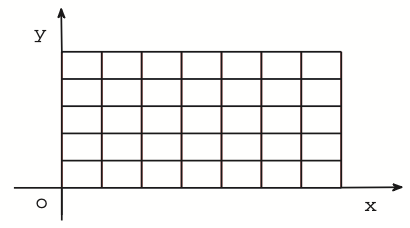
\includegraphics[width=0.45\textwidth]{fig/1.3.png}
    \captionof{figure}{二维网格示意图}
\end{figure}

将相应的内点集和边界点集分别记为
\begin{align*}
    &{\color{red} \Omega_h = \{(x_i, y_j) : 1 \leq i \leq I, 1 \leq j \leq J\}, } \\
    &{\color{red} \partial\Omega_h = \{(x_i, y_j) : i = 0 \text{ 或 } I+1, j = 0 \text{ 或 } J+1\}. }
\end{align*}

将其分类的原因是对于内格点，其满足微分方程，而对于外格点，直接使用边界条件即可.\par

现在将网格点上的连续信息离散化.
\begin{itemize}
    \item 当 $(x_i, y_j) \in \partial\Omega_h$ 时，有 $u_{ij} = \alpha(x_i, y_j) = \alpha_{ij}$；
    \item 当 $(x_i, y_j) \in \Omega_h$ 时，如下图所示，对二阶偏导均用二阶中心差商离散，
\end{itemize}


可得
\begin{equation*}
    \Delta_h u_{ij} := \frac{u_{i+1,j} - 2u_{ij} + u_{i-1,j}}{h^2} + \frac{u_{i,j+1} - 2u_{ij} + u_{i,j-1}}{k^2} = f(x_i, y_j) = f_{ij}.
\end{equation*}
故得求解 Poisson 方程 (2.1) 的五点差分格式如下:
\begin{equation}
    {\color{red} \left\{\begin{aligned}
        &\Delta_h u_{ij} = f_{ij}, \quad (x_i, y_j) \in \Omega_h, \\
        &u_{ij} = \alpha_{ij}, \quad (x_i, y_j) \in \partial\Omega_h.
    \end{aligned}\right.}
\end{equation}

\begin{figure}[H]
    \centering
    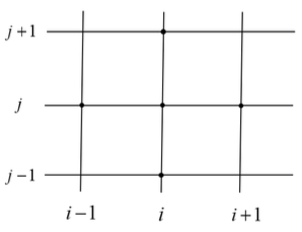
\includegraphics[width=0.35\textwidth]{fig/1.4.png}
    \captionof{figure}{五点差分格式节点示意图}
\end{figure}

\section{五点差分格式的性质}


\subsection{截断误差}
设 $u$ 为问题 (1.16) 的充分光滑解，$u_{ij}=u(x_i,y_j)$.\par
当$(x_i,y_j)\in\partial\Omega$时，$u_{ij}-\alpha_{ij}=0$.\par
当$(x_i,y_j)\in\Omega$时，由截断误差的定义知
\begin{align*}
    R_h u_{ij} &= \frac{u(x_i + h, y_j) - 2u(x_i, y_j) + u(x_i - h, y_j)}{h^2} \\
    &\quad + \frac{u(x_i, y_j + k) - 2u(x_i, y_j) + u(x_i, y_j - k)}{k^2} - f(x_i, y_j) \\
    &=: \mathrm{I}_1 + \mathrm{I}_2 - \Delta u(x_i, y_j).
\end{align*}

根据 Taylor 展开有
\begin{align*}
    u(x_i \pm h, y_j) =& u(x_i, y_j) \pm h u_x(x_i, y_j) + \frac{1}{2}h^2 u_{xx}(x_i, y_j) \\
    &\pm \frac{1}{3!}h^3 u_{xxx}(x_i, y_j) + \frac{1}{4!}h^4 u_{xxxx}(x_i + \xi_{\pm} h, y_j), \quad |\xi_{\pm}| < 1.
\end{align*}
于是
\begin{align*}
    \mathrm{I}_1 &= u_{xx}(x_i, y_j) + \frac{1}{12}h^2 \times \frac{1}{2}\{u_{xxxx}(x_i + \xi_+ h, y_j) + u_{xxxx}(x_i + \xi_- h, y_j)\} \\
    &= u_{xx}(x_i, y_j) + \frac{1}{12}h^2 u_{xxxx}(x_i + \xi h, y_j), \quad |\xi| < 1.
\end{align*}

类似可知，
\begin{align*}
    u(x_i, y_j \pm k) =& u(x_i, y_j) \pm k u_y(x_i, y_j) + \frac{1}{2}k^2 u_{yy}(x_i, y_j) \\
    &\pm \frac{1}{3!}k^3 u_{yyy}(x_i, y_j) + \frac{1}{4!}k^4 u_{yyyy}(x_i, y_j + \eta_{\pm} k), \quad |\eta_{\pm}| < 1.
\end{align*}

\begin{equation*}
    \mathrm{I}_2 = u_{yy}(x_i, y_j) + \frac{1}{12}h^2 u_{yyyy}(x_i, y_j + \eta k), \quad |\eta| < 1. 
\end{equation*}

所以，差分格式 (1.17) 的截断误差为
\begin{equation}
    R_h u_{ij} = \frac{1}{12} \left\{ h^2 u_{xxxx}(x_i, y_j + \xi h) + k^2 u_{yyyy}(x_i, y_j + \eta k) \right\}, \quad |\xi|, |\eta| < 1. 
\end{equation}

\subsection{存在唯一性}
问题：如何得到(1.17)的矩阵描述?若要深入研究，我们需要Kronecker张量积以及矩阵的拉直运算.但同时，我们也存在一些较为基础的方法.\par
若$(1.17)$可以写成$\bm{A}\vv{x}=\vv{u}$的形式，其解存在唯一$\iff$若$\vv{f}=\vv{0}$，则$\vv{u}=\vv{0}$.\par
将其离散化，若$f_{ij}=0,\alpha_{ij}=0$，能否得到$u_{ij}=0$，这一结构提示我们需要使用2维形式的离散极值原理.

\begin{lemma}[离散极值原理]
    设 $u_{ij}$ 是定义在 $\Omega_h \cup \partial\Omega_h$ 上的格点函数，
    \begin{enumerate}[label=(\arabic*)]
        \item 如果当 $(x_i, y_j) \in \Omega_h$ 时 $\Delta_h u_{ij} \geq 0$，则成立
        \begin{equation}
            \max_{\Omega_h} u_{ij} \leq \max_{\partial\Omega_h} u_{ij}. 
        \end{equation}
        \item 如果当 $(x_i, y_j) \in \Omega_h$ 时 $\Delta_h u_{ij} \leq 0$，则成立
        \begin{equation}
            \min_{\partial\Omega_h} u_{ij} \leq \min_{\Omega_h} u_{ij}. 
        \end{equation}
    \end{enumerate}
\end{lemma}
\begin{proof}
    用反证法证明 (1.19). 假设 (1.19) 不成立，则存在 $(x_{i_0}, y_{j_0}) \in \Omega_h$ 使得
    \begin{equation}
        M = \max_{\Omega_h} u_{ij} = u_{i_0 j_0} > \max_{\partial\Omega_h} u_{ij}. 
    \end{equation}
    在 $(x_{i_0}, y_{j_0})$ 处考察差分方程 (1.17) 有
    \begin{equation*}
        \Delta_h u_{i_0 j_0} = \frac{1}{h^2} \{u_{i_0+1, j_0} - 2u_{i_0 j_0} + u_{i_0-1, j_0}\} + \frac{1}{k^2} \{u_{i_0, j_0+1} - 2u_{i_0 j_0} + u_{i_0, j_0-1}\} \geq 0,
    \end{equation*}
    即
    \begin{equation*}
        2\left(\frac{1}{h^2} + \frac{1}{k^2}\right) M \leq \frac{1}{h^2} \{u_{i_0+1, j_0} + u_{i_0-1, j_0}\} + \frac{1}{k^2} \{u_{i_0, j_0+1} + u_{i_0, j_0-1}\}.
    \end{equation*}
    若格点函数 $u_{ij}$ 在 $(x_{i_0}, y_{j_0})$ 的某一相邻格点的函数值小于 $M$，则与上一不等式矛盾. 故有
    \begin{equation*}
        u_{i_0, j_0+1} = u_{i_0, j_0-1} = u_{i_0+1, j_0} = u_{i_0-1, j_0} = M.
    \end{equation*}
    对以上四邻点 (如仍为 $\Omega_h$ 中的格点) 进行同样推理，反复进行该过程，最后必能找到某边界格点 $(x_{i_1}, y_{j_1}) \in \partial\Omega_h$ 使得 $u_{i_1 j_1} = M$，这与假设 (1.21) 相矛盾.
\end{proof}

\begin{lemma}[连续情形极值原理]
    若在单连通区域 $\Omega$ 中成立 $\Delta u \geq 0$，可知
    \begin{equation}
        \max_{\bar{\Omega}} u = \max_{\partial\Omega} u. 
    \end{equation}
\end{lemma}



\begin{theorem}[]
    差分格式 (1.17) 之解存在唯一.
\end{theorem}
\begin{proof}
    只须证明若格点函数 $u_{ij}$ 满足$f_{ij}=0,\alpha_{ij}=0\Rightarrow u_{ij}=0$即可.\par
    当$(x_i,y_j)\in\Omega_h$时，$\Delta_h u_{ij}=0$，即$\Delta_h u_{ij}\geq 0,(x_i,y_j)\in \Omega_h$.\par
    故$\max_{\overline{\Omega_h}}u_{ij}=\max_{\partial\Omega_h}{u_{ij}}=\max_{\partial\Omega_h}\alpha_{ij}=0$.\par
    类似可知，$\min_{\overline{\Omega_h}}{u_{ij}}=0$.\par
    因此$u_{ij}\equiv 0$，得证.
\end{proof}

\subsection{收敛性}

\begin{theorem}[离散最大模估计]
    设 $u_{ij}$ 为定义在 $\Omega_h \cup \partial\Omega_h$ 上的格点函数，则
    \begin{equation*}
        \max_{\Omega_h} |u_{ij}| \leq \max_{\partial\Omega_h} |u_{ij}| + \frac{1}{2}a^2 \max_{\Omega_h} |\Delta_h u_{ij}|.
    \end{equation*}
\end{theorem}
\begin{proof}
    设 $A = \max_{\Omega_h} |\Delta_h u_{ij}|$. 构造辅助格点函数
    \begin{equation}
        w_{ij}^{\pm} = \pm u_{ij} + \frac{1}{2} x_i^2 A
    \end{equation}
    则有
    \begin{equation*}
        \Delta_h w_{i,j}^{\pm} = \pm \Delta_h u_{ij} + A \geq 0.
    \end{equation*}
    由离散极值原理即知
    \begin{equation*}
        \max_{\Omega_h} w_{ij}^{\pm} \leq \max_{\partial\Omega_h} w_{ij}^{\pm} \leq \max_{\partial\Omega_h} \left\{ \pm u_{ij} + \frac{A a^2}{2} \right\} \leq \max_{\partial\Omega_h} |u_{ij}| + \frac{A a^2}{2},
    \end{equation*}
    所以，
    \begin{equation*}
        \max_{\Omega_h} (\pm u_{ij}) \leq \max_{\partial\Omega_h} |u_{ij}| + \frac{1}{2}a^2 A \implies \max_{\Omega_h} |u_{ij}| \leq \max_{\partial\Omega_h} |u_{ij}| + \frac{1}{2}a^2 A.
    \end{equation*}
\end{proof}
对应的连续情形的极值估计为
\begin{theorem}[连续最大模估计]
    \[\max_{\Omega} |u(x,y)| \leq \max_{\partial\Omega} |u(x,y)| + \frac{1}{2}a^2 \max_{\Omega} |\Delta u(x,y)|.\]
\end{theorem}
由连续的最大模估计可知，设$\begin{cases}
\Delta u_1=f_1 \\
u_1=\alpha_1
\end{cases}$，$\begin{cases}
\Delta u_2=f_2 \\
u_2=\alpha_2
\end{cases}$.\par
将两式相减可得$\begin{cases}
\Delta(u_1-u_2)=f_1-f_2 \\
u_1-u_2=\alpha_1-\alpha_2
\end{cases}$，由连续的最大模估计可知
\begin{equation*}
    \max_{\Omega} |u_1 - u_2| \leq \max_{\partial\Omega} |\alpha_1 - \alpha_2| + \frac{1}{2}a^2 \max_{\Omega} |f_1 - f_2|.
\end{equation*}
这说明当边界条件和方程右端的函数发生微小变化时，解的变化也是微小的，即问题 (1.16) 是稳定的.\par

\subsection*{拓展}

可以通过待定系数方法来给出辅助格点函数的构造.\par
定义格点函数
\begin{equation*}
    w_{ij}^{\pm} = \pm u_{ij} + {\color{red}\phi_{ij}} A,
\end{equation*}
其中 $\phi = \phi(x,y)$ 是待定函数. 我们希望选取合适的 $\phi$ 使得 $w_{ij}^{\pm}$ 满足离散最大值原理，即 $\Delta_h w_{ij}^{\pm} \geq 0$. 直接计算有
\begin{equation*}
    \Delta_h w_{ij}^{\pm} = \pm \Delta_h u_{ij} + (\Delta_h \phi_{ij}) A.
\end{equation*}
注意到 $\pm \Delta_h u_{ij} + A \geq 0$，若要求
\begin{equation}
    {\color{red} \Delta_h \phi_{ij} \geq 1,} \tag{3.7}
\end{equation}
则
\begin{equation*}
    \Delta_h w_{ij}^{\pm} = \pm \Delta_h u_{ij} + (\Delta_h \phi_{ij}) A \geq 0.
\end{equation*}
在此情形下，有
\begin{equation*}
    \max_{\Omega_h} w_{ij}^{\pm} \leq \max_{\partial\Omega_h} w_{ij}^{\pm} = \max_{\partial\Omega_h} \{\pm u_{ij} + \phi_{ij} A\} \leq \max_{\partial\Omega_h} |u_{ij}| + (\max_{\partial\Omega_h} \phi_{ij}) A,
\end{equation*}
从而
\begin{align*}
    \max_{\Omega_h} |u_{ij}| &= \max_{\Omega_h} (\pm u_{ij}) = \max_{\Omega_h} (w_{ij}^{\pm} - \phi_{ij} A) \\
    &\leq \max_{\Omega_h} w_{ij}^{\pm} + (\max_{\Omega_h} (-\phi_{ij})) A \\
    &\leq \max_{\partial\Omega_h} |u_{ij}| + \alpha_h A = \max_{\partial\Omega_h} |u_{ij}| + \alpha_h \max_{\Omega_h} |\Delta_h u_{ij}|,
\end{align*}
式中
\begin{equation*}
    \alpha_h = \max_{\partial\Omega_h} \phi_{ij} + \max_{\Omega_h} (-\phi_{ij}).
\end{equation*}
显然可在式 (3.6) 中取
\begin{equation*}
    \phi(x,y) = \frac{1}{2}x^2, \quad (x,y) \in \bar{\Omega}.
\end{equation*}
事实上，二阶中心差商对三次多项式是精确的，所以 $\Delta_h \phi_{ij} = 1$，满足条件 (3.7)，且有
\begin{equation*}
    \max_{\Omega_h} |u_{ij}| \leq \max_{\partial\Omega_h} |u_{ij}| + \frac{1}{2}a^2 \max_{\Omega_h} |\Delta_h u_{ij}|.
\end{equation*}
若选取
\begin{equation*}
    \phi(x,y) = \frac{1}{4}(x^2 + y^2 - x - y), \quad (x,y) \in \bar{\Omega} = [0, a] \times [0, b],
\end{equation*}
且设 $a = b = 1$，则有 $\Delta_h \phi_{ij} = 1$，且成立
\begin{equation*}
    \max_{\Omega_h} |u_{ij}| \leq \max_{\partial\Omega_h} |u_{ij}| + \frac{1}{8} \max_{\Omega_h} |\Delta_h u_{ij}|.
\end{equation*}


